\section{Block boolean flags technique in the Generate phase (BBF)}

% Explains the generation phase 
% We can omit the explanation part, we can start in 'We observed...'
The EMS-GT algorithm follows the pattern-driven approach where it exhaustively tests the $4^l$ bit-array of possible motifs. As discussed earlier, EMS-GT quickly filters the $4^l$ bit-array in the Generate phase by intersecting the $d$-neighborhood of the first $n'$ sequences. EMS-GT maintains two $4^l$ bit-array during the Generate phase. The first array stores the remaining candidate motifs $\mathcal{C}$ and the second array stores the $d$-neighborhood of the current sequence $\mathcal{N}$. For every sequence in the first $n'$ sequences, we generate its $d$-neighborhood by blocks of bits settings. Then we intersect the $d$-neighborhood of the sequence with the candidate motifs array, the result will become the new candidate motifs array. We observed that at some point in the Generation phase, candidate motifs array has numerous empty blocks of $l$-mers. Applying block bits setting in this part of the neighborhood array will be useless since we already know that there is no candidate motifs in that block. An efficient way is to focus the neighborhood generation on those blocks where there are still candidate motifs. We have implemented a block boolean flags technique that tracks these empty blocks in the candidate motifs array.

\subsection{Maintaining block boolean flags for the candidate motifs array}
We divide the candidate motifs array $\mathcal{C}$ into groups of $4^k$ $l$-mers. The $k$ value should be the same with the one used in the block neighborhood generation strategy. In this study, we used $k = 5$. For each group of $4^k$ $l$-mers, we assigned a boolean flag that tells if the group is empty or not. Everytime we update the contents of the candidate motif array, we also update the boolean flags for empty blocks in the candidate motifs array. Given a candidate motifs array of size $4^l/32$, we maintain an array of block boolean flags $\mathcal{B}$ of size $(4^l/32)/(4^k/32)$. Figure \ref{fig:boolean-flags} illustrates the way of grouping these $4^k$ $l$-mers and its corresponding block boolean flags.

Formally, for any row value $v$ and block height value $h$, the block boolean flags array is defined as:
\begin{equation}
	\mathcal{B}[v] = \left\{
		\begin{array}{rl}
			1 & \text{if candidate motif exists in } \mathcal{C}[v * h, (v * h) + h), \\
			0 & \text{otherwise.}
		\end{array} \right. 
	% \text{ for any row value }v \text{ and block height value }h. \\
\end{equation}

\begin{figure}[h]
	\centering
	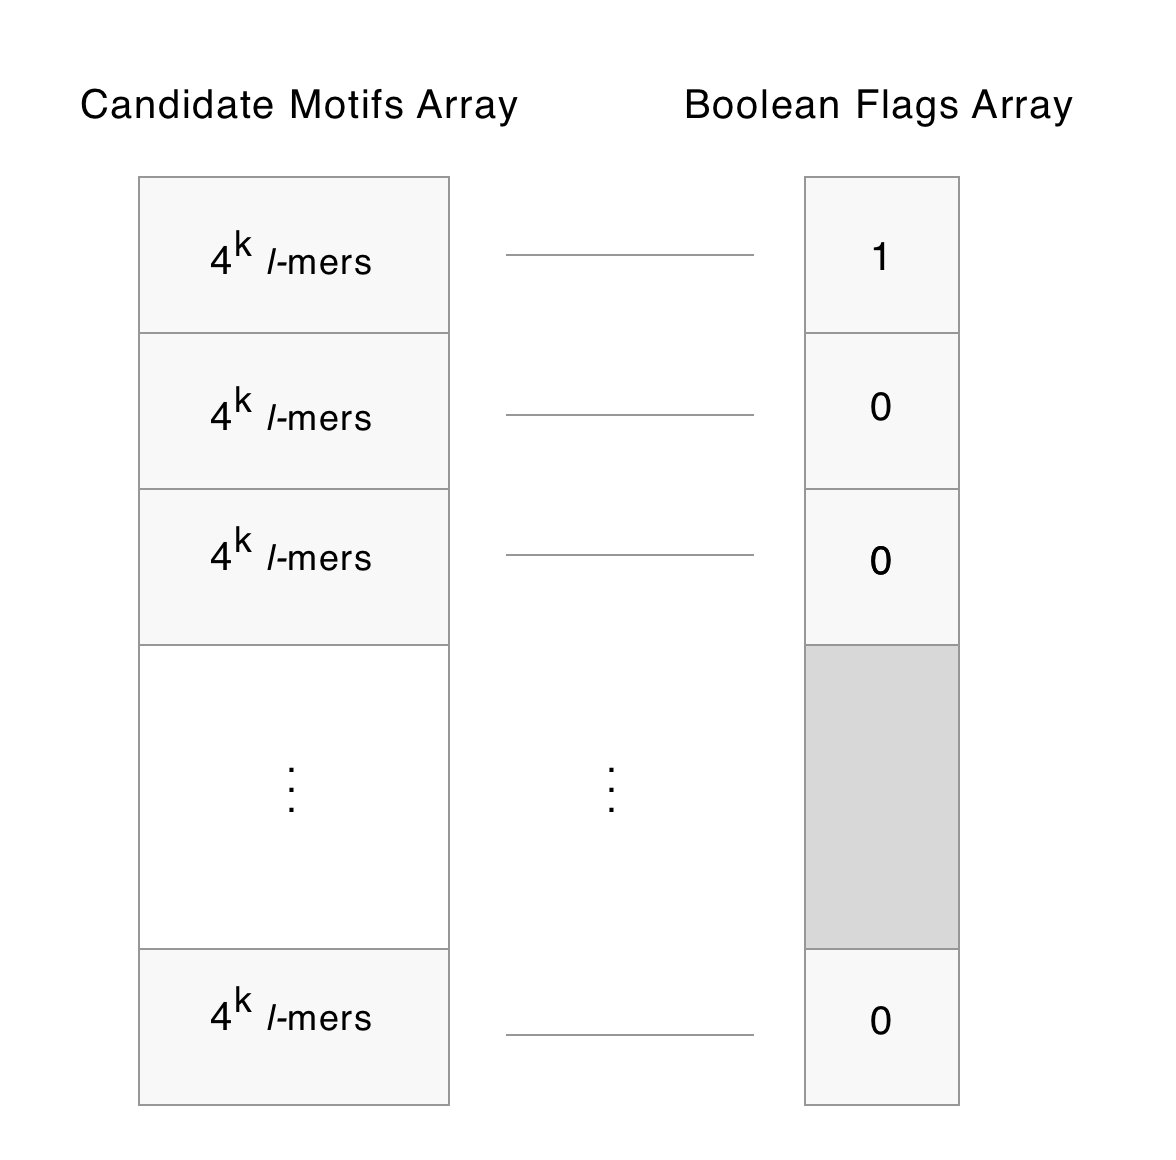
\includegraphics[width=3.5in]{contents/00_images/boolean-flags}\vspace*{5pt}
	
	\caption{Assigning boolean flags for every $4^k$ $l$-mers block in the candidate motifs array.}
	\label{fig:boolean-flags}
\end{figure}

\subsection{Usage of block boolean flags strategy}

The improved $d$-neighborhood generation of $l$-mer uses a pre-generated block patterns of size $4^k$ $l$-mers. Given these patterns, we recursively generate all possible prefix, with length $l - k$, of the given $l$-mer. These prefix values represents the row start value where the block bits setting will be applied. For each prefix value, we check if can skip the block bits setting by checking if the block is empty using its assigned block boolean flag. If the prefix value is not equal to the row start value of the block the boolean flag is representing, then we need to also check the next boolean flag if it is empty since the block bits setting will overlap, unless it is the last block in the array. Figure \ref{fig:boolean-block-skip} shows an illustration for these scenarios.

% Figure 4.\ref{fig:boolean-block-skip} shows scenarios in checking the block boolean flag. The first scenario is a block bits setting that has a prefix value of 0, since there will be no overlap we only have to consider its corresponding boolean flag. The second scenario has a prefix value of 25, this case we also have to consider the next boolean flag if it is empty or not before skipping the block bits setting.

\begin{figure}[h]
	\centering
	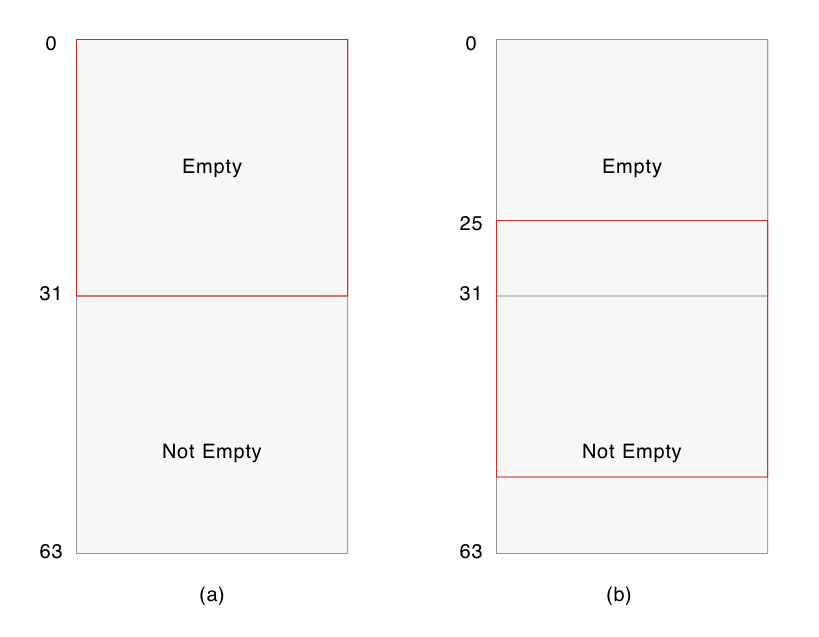
\includegraphics[width=3.5in]{contents/00_images/block-skip}\vspace*{5pt}
	\caption{(a) Shows a skipped block bit setting with prefix value of 0; (b) Shows a block bit setting with prefix value of 25.}
	\label{fig:boolean-block-skip}
\end{figure}

% Make this the last paragraph
Block boolean flags strategy checks if a block is not empty before applying the block bits setting. This approach is useful when there are sufficiently large number of empty blocks in the candidate motifs array. We introduced a new parameter $n''$, where $1 < n'' < n'$, that is the sequence number where we will start using the block boolean flags strategy. In this study, we use for problem instances (9, 2), (11, 3), (13, 4), (15, 5) and (17, 6) the $n''$ value of 8, 10, 7, 7 and 7 respectively.



